\section{}
\subsection*{(a)}

$G$ and $H$ share the same set of minimum spanning trees. First it must be proved that any minimum spanning tree for $G$ is also a minimum spanning tree for $H$ and then it must be proved that any minimum spanning tree for $H$ is also a minimum spanning tree for $G$.

Let $w_g(graph)$ be the summation of all weights of a tree in the graph $G$, and $w_h(graph)$ be the summation of all weights of a tree in the graph $H$.
Let $T$ be a minimum spanning tree for $G$

\textbf{Proof:}

Recall, by properties of a MST, an MST for $G$ or $H$ will have $V-1$ edges. Because each edge in $H$ has a weight that is $1$ greater than the weight in $G$, $w_h\left(T\right)=\ w_g\left(T\right)+(V-1)$
\textbf{ATAC:} Assume there is a minimum spanning tree $A$ for the graph $H$ that is not a minimum spanning tree for $G$. By definition, $w_g\left(A\right)>w_g\left(T\right)$ and $w_h\left(A\right)\le w_h\left(T\right)$.

\begin{eqnarray}
    w_g\left(A\right)>w_g\left(T\right) \\
    w_h\left(A\right)-\left(V-1\right)>w_h\left(T\right)-(V-1)
\end{eqnarray}
The $-(V-1)$ terms cancel:
\begin{equation}
    w_h\left(A\right)>w_h\left(T\right)
\end{equation}
But by definition:
\begin{equation}
    w_h\left(A\right)\le w_h\left(T\right)
\end{equation}
Contradiction! If $A$ is not a minimum spanning tree of $G$, it also cannot be a minimum spanning tree for $H$.

\textbf{ATAC:} Assume there is a minimum spanning tree $B$ for the graph $G$ that is not a minimum spanning tree for $H$. By definition, $w_h\left(B\right)>w_h\left(T\right)$ and $w_g\left(B\right)\le w_g\left(T\right)$.
\begin{eqnarray}
    w_h\left(B\right)>w_h\left(T\right) \\
    w_g\left(B\right)+(V-1)>w_g\left(T\right)+(V-1)
\end{eqnarray}
The $+(V-1)$ terms cancel:
\begin{eqnarray}
    w_g\left(B\right)>w_g\left(T\right)
\end{eqnarray}
But by definition:
\begin{eqnarray}
    w_g\left(B\right)\le w_g\left(T\right)
\end{eqnarray}
Contradiction! If $B$ is not a minimum spanning tree of $H$, it also cannot be a minimum spanning tree for $G$.

This means that there cannot be any graph that is a minimum spanning tree for $H$ but not $G$ or a minimum spanning tree for $G$ but not $H$.

Therefore, $G$ and $H$ share the same set of minimum spanning trees.


\subsection*{(b)}

$G$ and $H$ do not always share the same shortest path between all pairs of vertices.

Consider the following graph $G$

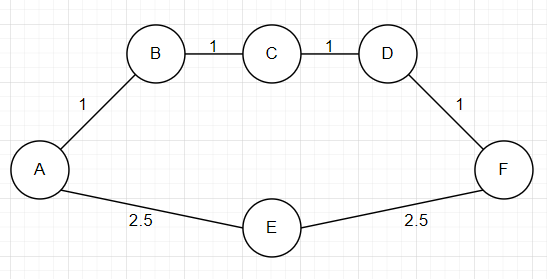
\includegraphics[width=\textwidth]{Picture1.png}

The shortest path from A → F is: A → B → C → D → F, having a total weight of 4.
This same graph in H becomes:

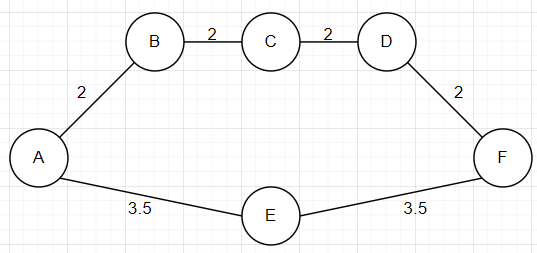
\includegraphics[width=\textwidth]{Picture2.png}

Now the path A → B → C → D → F has weight 8, while the path A → E → F has weight 7. This means that the shortest path A → F is A → E → F. This counter example proves that G and H do not always share the same shortest path between all pairs of vertices.